\chapter{Shor's Algorithm}
\section{Introduction}
The most spectacular discovery in quantum computing to date is that quantum computers can effectively perform some tasks that are not feasible on a classical computer. For example, finding the prime factorization of an $n$-bit integer is thought to require $exp(\Theta(n^{1/3}\log^{2/3} n))$ operations using the best classical algorithm known at the time of writing — the so-called number field sieve. This is exponential in the size of the number being factored, so factoring is generally considered to be an intractable problem on a classical computer: it quickly becomes impossible to factor even modest-sized numbers. In contrast, a quantum algorithm can accomplish the same task using $O(n^2 \log n \log \log n)$ operations. That is, a quantum computer can factor a number exponentially faster than the best known classical algorithms. This result is important in its own right, but perhaps the most exciting aspect is the question it raises: what other problems can be solved efficiently on a quantum computer that are infeasible on a classical computer?

We can now factor integers efficiently using quantum computers, and this is the problem solved by Shor's algorithm. Really, it turns out that ``Shor's algorithm" is more of a technique than a specific algorithm, and it can be used to solve an interesting collection of problems. (Order finding is one of the simplest to describe.)

\section{Problem Definition}
\begin{definition}
    \textbf{Input:} Given a number $N \geq 2$ which is a composite number. \\
    \textbf{Output:} We are required to find the prime factorization of the number $N = p_1^{k_1} \ldots p_m^{k_m}$.
\end{definition}


Let us note a few facts, which we will not prove or discuss in any detail. First, if $N$ is a prime number or a prime power (i.e., $p^k$ for some prime $p$ and integer $k \geq 1$), then there are efficient classical algorithms for solving the integer factorization problem in these cases. So, we can imagine that we first run such an algorithm on the input $N$; if it succeeds, then we are done. Otherwise, we continue under the assumption that $N$ has at least two distinct prime factors (i.e., $m \geq 2$).

Next, it is enough to have an algorithm that takes a composite $N$ as input and just finds two integers $u, v \geq 2$ such that $N = uv$. If we have such an algorithm, we can run it recursively (interleaved with the classical algorithm for prime powers) to find a complete prime factorization of $N$.

Finally, if our goal is to find integers $u, v \geq 2$ such that $N = uv$ for $N$ an even composite number, then we really don't need to work very hard; let $u = 2$ and $v = N/2$.

Now, consider the process described as follows. The basic idea is as follows. Suppose that the random choice of $a \in \mathbb{Z}_N^*$ (which is very likely), and that the order of $a$ is even. Then
\[
a^r \equiv 1 \pmod{N}
\]
so
\[
N \mid a^r - 1
\]
Because $a^r - 1 = (a^{r/2} + 1)(a^{r/2} - 1)$, we have
\[
N \mid (a^{r/2} + 1)(a^{r/2} - 1)
\]
It cannot happen that $N \mid (a^{r/2} - 1)$, because this would mean that $r$ was not the order of $a$ after all. If we are lucky and it is not the case that $N \mid (a^{r/2} + 1)$, then we know the algorithm will work. This is because the factors of $N$ are then necessarily split between $(a^{r/2} + 1)$ and $(a^{r/2} - 1)$, so computing $\gcd(a^{r/2} - 1, N)$ will reveal a nontrivial factor of $N$.

Each iteration of the loop therefore fails to give an answer if either $r$ is odd, or $r$ is even but $N$ divides $a^{r/2} + 1$. The probability that neither of these events occurs is at least $1/2$. (In fact, it is at least $1 - 2^{1 - m}$ for $m$ the number of distinct primes dividing $N$.) This is why the assumption that $N$ is not a prime power was important. Also, the analysis of this fact requires that $N$ is odd.


\section{Idea of the Algorithm}

Let us now see that the integer factoring problem can be efficiently solved given an algorithm for order-finding. A fast algorithm for order-finding can easily be turned into a fast algorithm for factoring. In other words, factoring reduces to order-finding. To be specific, it is a randomized polynomial-time Turing reduction — the type of reduction you might have seen. The idea, however, is essentially the same: if you have an efficient algorithm for order-finding, then the reduction gives you an efficient algorithm for factoring.

To demonstrate this reduction, suppose we are given an $n$-bit composite number $N = pq$, where $p$ and $q$ are distinct primes, and our goal is to efficiently determine the factors $p$ and $q$. 

\begin{enumerate}
    \item Pick a random integer $a \in \mathbb{Z}_N^*$, i.e., $1 < a < N$ and $\gcd(a, N) = 1$.
    \item Use an order-finding algorithm (quantum, in our case) to compute $r = \operatorname{ord}_N(a)$.
\end{enumerate}

Now, since $a^r \equiv 1 \pmod{N}$ by definition of order, it follows that $a^r - 1 \equiv 0 \pmod{N}$, so $N$ divides $a^r - 1$:
\[
N \mid a^r - 1.
\]
If $r$ is even, we can write:
\[
a^r - 1 = \left(a^{r/2} - 1\right)\left(a^{r/2} + 1\right),
\]
which is the difference of squares. Because $N = pq$ divides this product, it must be that both $p$ and $q$ divide either of the two factors. However, since $r$ is the smallest number such that $a^r \equiv 1 \pmod{N}$, it cannot be that both $p$ and $q$ divide $a^{r/2} - 1$, or else $r$ would not be minimal.

Thus, we are left with three distinct possibilities:
\begin{enumerate}
    \item $p \mid a^{r/2} - 1$ and $q \mid a^{r/2} + 1$,
    \item $q \mid a^{r/2} - 1$ and $p \mid a^{r/2} + 1$,
    \item Both $p$ and $q$ divide $a^{r/2} + 1$.
\end{enumerate}

In the first two cases, $p$ and $q$ divide different factors, which is exactly what we want. We can then compute:
\[
\gcd(a^{r/2} - 1, N) \quad \text{or} \quad \gcd(a^{r/2} + 1, N),
\]
to recover one of the prime factors. If either of these greatest common divisors yields a non-trivial factor of $N$, we have successfully factored $N$.


\begin{definition}
    \textbf{(Lucky element in $\mathbb{Z}_N^*$)}.  
    Let $N \geq 2$. An element $a \in \mathbb{Z}_N^*$ is said to be \emph{lucky} if the order $r = \operatorname{ord}_N(a)$ is even and $N$ does not divide $a^{r/2} + 1$. In such cases, the reduction from order-finding to factoring succeeds.
\end{definition}

Given a lucky $a \in \mathbb{Z}_N^*$, we can compute:
\[
\gcd(a^{r/2} + 1,\, N) \in \{p, q\} \qquad \text{or} \qquad \gcd(a^{r/2} - 1,\, N) \in \{p, q\},
\]
which yields a non-trivial factor of $N$. The value $a^{r/2}$ can be computed efficiently using the method of repeated squaring (recall section~\ref{subsec:repeated_squaring_trick}), with a gate cost of $\mathcal{O}(n^2 \log n)$ for $n$-bit integers.

The only remaining challenge is how to find such a lucky $a \in \mathbb{Z}_N^*$. Unfortunately, no deterministic method is known for selecting a lucky element. However, it is known that for any $N = pq$, where $p$ and $q$ are distinct primes, a large fraction of elements in $\mathbb{Z}_N^*$ are lucky.

\begin{lemma}
    For all integers $N = pq$, where $p$ and $q$ are distinct primes, at least half of the elements $a \in \mathbb{Z}_N^*$ are lucky.
\end{lemma}

This means that choosing a random $a \in \mathbb{Z}_N^*$ will result in a lucky value with probability at least $\frac{1}{2}$. Consequently, the factoring algorithm succeeds with probability at least $\frac{1}{2}$ on each attempt. The success probability can be amplified by repeating the procedure multiple times with independently chosen values of $a$.

If the chosen $a$ is unlucky (i.e., $r$ is odd, or $a^{r/2} \equiv -1 \pmod{N}$), we simply discard it and choose another random $a$. Since the probability of success is high, only a small number of iterations are typically needed.

In summary, an efficient algorithm for the order-finding problem yields an efficient algorithm for factoring integers of the form $N = pq$. This is highly significant, since the security of widely used cryptographic systems such as RSA relies on the hardness of factoring large integers. In the next section, we turn our attention to developing an efficient quantum algorithm for solving the order-finding problem.


\section{Reduction of factoring to order-finding}

The reduction of factoring to order-finding proceeds in two basic steps. The first step is to show that we can compute a factor of $N$ if we can find a non-trivial solution $x \not\equiv \pm 1 \pmod{N}$ to the equation $x^2 \equiv 1 \pmod{N}$. The second step is to show that a randomly chosen $y$ co-prime to $N$ is quite likely to have an order $r$ which is even, and such that $y^{r/2} \not\equiv \pm 1 \pmod{N}$, and thus $x \equiv y^{r/2} \pmod{N}$ is a non-trivial solution to $x^2 \equiv 1 \pmod{N}$. These two steps are embodied in the following theorems.

\begin{theorem}
    Suppose $N$ is an $L$-bit composite number, and $x$ is a non-trivial solution to the equation $x^2 \equiv 1 \pmod{N}$ in the range $1 \leq x \leq N$, that is, neither $x \equiv 1 \pmod{N}$ nor $x \equiv -1 \pmod{N}$. Then at least one of $\gcd(x - 1, N)$ and $\gcd(x + 1, N)$ is a non-trivial factor of $N$ that can be computed using $\mathcal{O}(L^3)$ operations.
\end{theorem}

\begin{theorem}
    Suppose $N = p_1^{\alpha_1} \ldots p_m^{\alpha_m}$ is the prime factorization of an odd composite positive integer. Let $x$ be an integer chosen uniformly at random, subject to the requirements that $1 \leq x \leq N - 1$ and $x$ is co-prime to $N$. Let $r$ be the order of $x$ modulo $N$. Then
    \[
    \Pr\left(r \text{ is even and } x^{r/2} \not\equiv -1 \pmod{N} \right) \geq 1 - \frac{1}{2^m}.
    \]
\end{theorem}

Both these theorems can be combined to give an algorithm which, with high probability, returns a non-trivial factor of any composite $N$. All the steps in the algorithm can be performed efficiently on a classical computer, except (so far as is known today) the order-finding \emph{subroutine}, which is used by the algorithm. By repeating the procedure, we may find a complete prime factorization of $N$. The algorithm is summarized as follows:

\begin{algorithm}
    \caption{Shor's Algorithm}
    \begin{algorithmic}[1]
    \State \textbf{Input:} A composite number $N$
    \State \textbf{Output:} A non-trivial factor of $N$
    \State \textbf{Runtime: } $\mathcal{O}((\log N)^3)$ operations. Succeeds with probability $\mathcal{O}(1)$.
    \State \begin{itemize}
        \item If $N$ is even, return the factor $2$.
        \item Determine whether $N = a^b$ for integers $a \geq 1$ and $b \geq 2$, and if so, return the factor $a$ (uses a classical algorithm).
        \item Randomly choose $x$ in the range $1$ to $N - 1$. If $\gcd(x, N) > 1$, then return the factor $\gcd(x, N)$.
        \item Use the order-finding subroutine to find the order $r$ of $x$ modulo $N$.
        \item If $r$ is even and $x^{r/2} \not\equiv -1 \pmod{N}$, then compute $\gcd(x^{r/2} - 1, N)$ and $\gcd(x^{r/2} + 1, N)$, and test whether one of these is a non-trivial factor, returning that factor if so. Otherwise, the algorithm fails.
    \end{itemize}
    \end{algorithmic}
\end{algorithm}

Steps 1 and 2 of the algorithm either return a factor or else ensure that $N$ is an odd integer with more than one prime factor. These steps may be performed using $\mathcal{O}(1)$ and $\mathcal{O}(L^3)$ operations, respectively. Step 3 either returns a factor or produces a randomly chosen element $x$ of $\{0,1,2,\ldots,N-1\}$. Step 4 calls the order-finding subroutine, computing the order $r$ of $x$ modulo $N$. Step 5 completes the algorithm, since theorems guarantee that with probability at least one-half, $r$ will be even and $x^{r/2} \not\equiv -1 \pmod{N}$, and then the theorem guarantees that either $\gcd(x^{r/2} - 1, N)$ or $\gcd(x^{r/2} + 1, N)$ is a non-trivial factor of $N$.


\begin{example}
    Suppose $N$ is $L$ bits long. The aim of this exercise is to find an efficient classical algorithm to determine whether $N = a^b$ for some integers $a \geq 1$ and $b \geq 2$. This may be done as follows:
    \begin{enumerate}
        \item Show that $b$, if it exists, satisfies $b \leq L$.
        \item Show that it takes at most $\mathcal{O}(L^2)$ operations to compute $\log_2 N$, $x = y/b$ for $b \leq L$, and the two integers $u_1$ and $u_2$ nearest to $2^x$.
        \item Show that it takes at most $\mathcal{O}(L^2)$ operations to compute $u_1^b$ and $u_2^b$ (using repeated squaring), and check to see if either is equal to $N$.
        \item Combine the previous results to give an $\mathcal{O}(L^3)$-operation algorithm to determine whether $N = a^b$ for integers $a$ and $b$.
    \end{enumerate}
\end{example}

\begin{example}
    \textbf{(Factoring 91)} Suppose we wish to factor $91$. Confirm that steps 1 and 2 are passed. For step 3, suppose we choose $x = 4$, which is co-prime to $91$. Compute the order $r$ of $x$ with respect to $N$, and show that $x^{r/2} \bmod 91 = 64 \not\equiv -1 \pmod{91}$, so the algorithm succeeds, giving $\gcd(64 - 1, 91) = 7$.\\
    It is unlikely that this is the most efficient method you've seen for factoring $91$. Indeed, if all computations had to be carried out on a classical computer, this reduction would not result in an efficient factoring algorithm, as no efficient method is known for solving the order-finding problem on a classical computer.
\end{example}

\begin{example}
    Show that $N = 15$ is the smallest number for which the order-finding subroutine is required — that is, it is the smallest composite number that is neither even nor a power of some smaller integer.
\end{example}

\section{Example}

The use of order-finding, phase estimation, and continued fraction expansions in the quantum factoring algorithm is illustrated by applying it to factor $N = 15$. First, we choose a random number that has no common factors with $N$; suppose we choose $x = 7$. Next, we compute the order $r$ of $x$ with respect to $N$ using the quantum order-finding algorithm: begin with the state $\ket{0}\ket{0}$ and create the state
\[
\frac{1}{\sqrt{2^t}} \sum_{k=0}^{2^t - 1} \ket{k}\ket{0} = \frac{1}{\sqrt{2^t}} [\ket{0} + \ket{1} + \ket{2} + \ldots + \ket{2^t - 1}]\ket{0}
\]
by applying $t = 11$ Hadamard transforms to the first register. Choosing this value of $t$ ensures an error probability $\epsilon$ of at most $1/4$. Next, compute $f(k) = x^k \bmod N$, leaving the result in the second register:
\[
\frac{1}{\sqrt{2^t}} \sum_{k=0}^{2^t - 1} \ket{k}\ket{x^k \bmod N}
\]
\[
= \frac{1}{\sqrt{2^t}} [\ket{0}\ket{1} + \ket{1}\ket{7} + \ket{2}\ket{4} + \ket{3}\ket{13} + \ket{4}\ket{1} + \ket{5}\ket{7} + \ket{6}\ket{4} + \ldots]
\]

We now apply the inverse Fourier transform $FT^{\dagger}$ to the first register and measure it. One way to analyze the distribution of outcomes is to calculate the reduced density matrix for the first register, apply $FT^{\dagger}$ to it, and calculate the measurement statistics. However, since no further operation is applied to the second register, we can instead apply the principle of implicit measurement and assume that the second register is measured, obtaining a random result from $\ket{1}, \ket{7}, \ket{4}$, or $\ket{13}$. Suppose we get $\ket{4}$ (any result works); this means the input to $FT^{\dagger}$ would have been
\[
\sqrt{\frac{4}{2^t}} [\ket{2} + \ket{6} + \ket{10} + \ket{14} + \ldots ].
\]

After applying $FT^{\dagger}$, we obtain a state $\sum_l \alpha_l \ket{l}$, with the probability distribution shown in Figure~\ref{fig:magplot} for $2^t = 2048$. The final measurement gives either $0, 512, 1024$, or $1536$, each with probability approximately $1/4$. Suppose we obtain $l = 1536$ from the measurement. Computing the continued fraction expansion gives $1536/2048 = 1/(1 + 1/3)$, so that $3/4$ occurs as a convergent in the expansion, yielding $r = 4$ as the order of $x = 7$.

By chance, $r$ is even, and moreover, $x^{r/2} \bmod N = 7^2 \bmod 15 = 4 \not\equiv -1 \pmod{15}$, so the algorithm works: computing the greatest common divisors $\gcd(x^2 - 1, 15) = 3$ and $\gcd(x^2 + 1, 15) = 5$ tells us that $15 = 3 \times 5$.

\begin{figure}[ht]
    \centering
    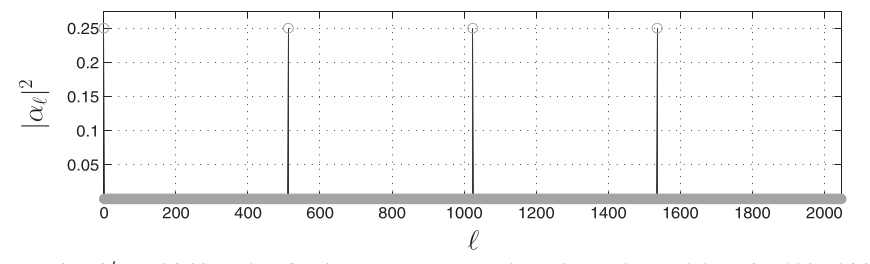
\includegraphics[width=1\linewidth]{Images/plotmagvsl.png}
    \caption{Plot of magnitude vs $l$}
    \label{fig:magplot}
\end{figure}


\section{Summary}

The algorithm samples uniformly from $\mathbb{Z}_m^*$ by sampling an $a$ uniformly from the simple set $\{1, 2, \ldots, m - 1\}$ and then checking whether or not $\gcd(a, m) = 1$. If $\gcd(a, m) = 1$, then $a \in \mathbb{Z}_m^*$ and the algorithm proceeds. If $\gcd(a, m) > 1$, then although the algorithm could randomly sample another element from $\{1, 2, \ldots, m - 1\}$, that's not necessary, because in that event, $\gcd(a, m)$ is a proper divisor of $m$.

In the event that $a \in \mathbb{Z}_m^*$, the probability that $a$ is lucky is at least $\frac{1}{2}$. If $a$ is lucky, then the algorithm computes $\gcd(a^{r/2} + 1, m)$ to obtain a factor of $m$. This part can be computed by repeated squaring and Euclid's algorithm.

The implementation cost of this algorithm is $\mathcal{O}(n^2 \log n)$ gates. Although we only analyzed this algorithm for the case where $m$ is the product of two distinct primes, it turns out that this factoring algorithm succeeds with probability at least $\frac{1}{2}$ for any number $m$ that's not a prime power. For the prime power case (where $m = p^k$ for a prime $p$), there's a simple classical algorithm. That algorithm can be run as a preprocessing step to this algorithm.

\begin{algorithm}
    \caption{Shor's Algorithm}
    \begin{algorithmic}[1]
    \State \textbf{Input:} A composite number $N$
    \State \textbf{Output:} A non-trivial factor of $N$
    \State \textbf{Runtime:} $\mathcal{O}((\log N)^3)$ operations. Succeeds with probability $\mathcal{O}(1)$.
    \State \begin{itemize}
        \item If $N$ is even, return the factor $2$.
        \item Determine whether $N = a^b$ for integers $a \geq 1$ and $b \geq 2$, and if so, return the factor $a$ (uses the classical algorithm).
        \item Randomly choose $x$ in the range $1$ to $N - 1$. If $\gcd(x, N) > 1$, then return the factor $\gcd(x, N)$.
        \item Use the order-finding subroutine to find the order $r$ of $x$ modulo $N$.
        \item If $r$ is even and $x^{r/2} \not\equiv -1 \pmod{N}$, then compute $\gcd(x^{r/2} - 1, N)$ and $\gcd(x^{r/2} + 1, N)$, and test whether one of these is a non-trivial factor, returning that factor if so. Otherwise, the algorithm fails.
    \end{itemize}
    \end{algorithmic}
\end{algorithm}








% \chapter{Period-finding}
% Consider the following problem. 
% \section{Problem Definition}
% Suppose $f$ is a periodic function producing a single bit as output such that $f(x+r)=f(x)$, for some unknown $0<r<2^L$, where $x,r\in\{0,1,2,\ldots\}$. Given a quantum black box $U$ which performs the unitary transform $U\ket{x}\ket{y}\rightarrow \ket{x}\ket{y\oplus f(x)}$ (where $\oplus$ denotes addition modulo $2$) how many black box queries and other operations are required to determine $r$? Note that in practice $U$ operates on a finite domain, whose size is determined by the desired accuracy of $r$. Here is a quantum algorithm which solve this problem using one query, and $\mathcal{O}(L^2)$ other operations.
% \begin{algorithm}
%     \caption{Period-finding Algorithm}
%     \begin{algorithmic}[1]
%     \State \textbf{Input:} (1) A black box which performs the operation $U\ket{x}\ket{y}=\ket{x}\ket{y\oplus f(x)}$, (2) a state to store the function evaluation initialized to $\ket{0}$, and (3) $t=\mathcal{O}(L+\log(1/2\epsilon))$ qubits initialized to $\ket{0}$.
%     \State \textbf{Output:} The least integer $r>0$ such that $f(x+r)=f(x)$.
%     \State \textbf{Runtime: } One use of $U$, and $\mathcal{O}(L^2)$ operations, succeeds with probability $\mathcal{O}(1)$.
%     \State \textbf{Procedure: }
%     \State \hspace{1em} \textbf{Initialize: }$\ket{0}\ket{0}$
%     \State \hspace{1em} \textbf{Create superposition: } $\rightarrow \frac{1}{\sqrt{2^t}}\sum_{x=0}^{2^t-1} \ket{x}\ket{0}$
%     \State \hspace{1em} \textbf{Apply $U$: }$\rightarrow \frac{1}{\sqrt{2^t}}\sum_{s=0}^{2^t-1} \ket{x}\ket{f(x)}\approx \frac{1}{\sqrt{r2^t}}\sum_{l=0}^{r-1}\sum_{x=0}^{2^t-1} e^{2\pi\iota lx/r}\ket{x}\ket{\hat{f}(l)}$
%     \State \hspace{1em} \textbf{Apply inverse Fourier transform to first register} $\rightarrow \frac{1}{\sqrt{r}}\sum_{l=0}^{r-1} \ket{\tilde{l/r}}\ket{\hat{f}(l)}$
%     \State \hspace{1em} \textbf{Measure first register:}$\rightarrow \tilde{l/r}$
%     \State \hspace{1em} \textbf{Apply continued fractions algorithm} $\rightarrow r$
%     \end{algorithmic}
% \end{algorithm}

% the key to understanding this algorithm, which is based on phase estimation, and is nearly identical to the algorithm for quantum order finding, is step 3, in which we introduce the state
% \[
% \ket{\hat{f}(l)}\equiv \frac{1}{\sqrt{r}}\sum_{x=0}^{r-1} e^{-2\pi\iota lx/r}\ket{f(x)}
% \]
% the Fourier transform of $\ket{f(x)}$. The identity used in step 3 is based on
% \[
% \ket{f(x)}=\frac{1}{\sqrt{r}}\sum-{l=0}^{r-1}e^{2\pi\iota lx/r}\ket{\hat{f}(l)}
% \]
% which is easy to verify by noting that $\sum_{l=0}^{r-1}e^{2\pi\iota lx/r}=r$ for $x$ an integer multiple of $r$, and zero otherwise. The approximate equality in step 3 is required because $2^t$ may not be an integer multiple of $r$ in general (it need not be: this is taken account of by the phase estimation bound). Applying the inverse Fourier transform to the first register, in step $4$, gives an estimate of the phase $l/r$, where $l$ is chosen randomly, $r$ can be efficiently obtained in the final step using a continued fraction expansion.











% \chapter{Hidden Subgroup problem}
% One of the general application of the quantum Fourier transform are general problem known as the hidden subgroup problem. We will now describe an efficient quantum algorithm for solving it. This problem, which encompasses all known `exponentially fast' application of the quantum Fourier transform, can be thought of as a generalization of the task of finding the unknown period of a periodic function, in a context where the structure of the domain and range of the function may be very intricate.


\chapterreferences
